\documentclass[a4paper, 11pt]{article}
\usepackage[utf8]{inputenc} % Change according your file encoding
\usepackage{graphicx}
\usepackage{url}
\usepackage{listings}

%opening
\title{Seminar Report: Paxy}
\author{Erkki Heino, Bastien Scanu}
\date{\today{}}

\begin{document}

\maketitle

\section{Introduction}

The PAXOS algorithm is a consensus protocol based on gaining votes from a quorum. In this protocol, processors may operate at an arbitrary speed and may crash, but cannot lie. Messages can take arbitrary long time to be delivered, get lost or duplicated but not corrupted. The different actors are the proposers, that suggest a value in order to agree on a single one, and the acceptors that will vote and decide the value to be agreed. We will implement this algorithm with Erlang.

\section{Work done}

We only had to fill the blanks in the code, so we didn't have to take important design decision. To split the paxy module in two parts, we had to...

\section{Experiments}

\subsection{Delay in the acceptors}
In this experiment, we will introduce some delays in the acceptors by adding a sleep function just after receiving prepare and receive messages. We added the following lines to the acceptor file:
\begin{lstlisting}
-define(delay, 20).
R = random:uniform(?delay),
timer:sleep(R),
\end{lstlisting}
We can see on Figure1 that the algorithm still terminates with a small number of rounds.
\begin{figure}[h!]
\begin{center}
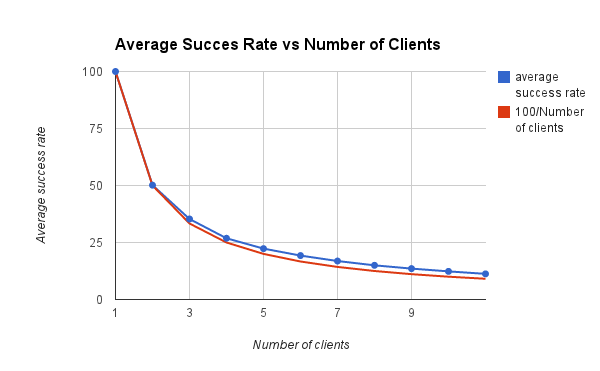
\includegraphics[scale=0.5]{exp1.jpg}
\caption{Result obtained with the 1st eperiment}
\end{center}
\end{figure}

\subsection{Ignore the sorry messages}
The second experiment consists in making the acceptors ignore the sorry messages, simply by commenting the corresponding code in the acceptor file. As we see in Figure2, it does not affect the algorithm, it still terminates and we come to an agreement in few rounds.
\begin{figure}[h!]
\begin{center}
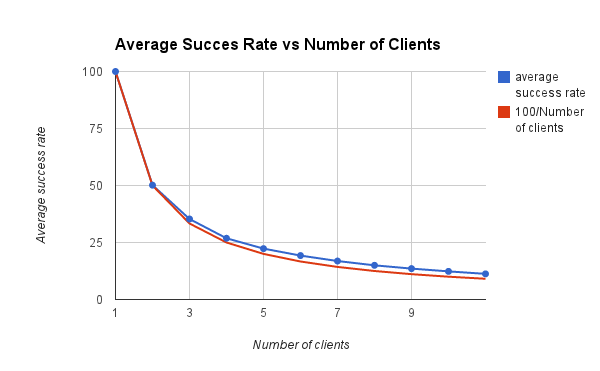
\includegraphics[scale=0.5]{exp1.jpg}
\caption{Result obtained with the 2nd eperiment}
\end{center}
\end{figure}

\subsection{Randomly drop messages}
We will now try to randomly drop some promise and vote messages and see how it affects the behavior of our algorithm. To implement this, we created the following function:
\begin{lstlisting}
-define(drop, 10).
send(Name, Message) ->
  case random:uniform(?drop) of
    ?drop ->
      io:format("message dropped~n");
    _ ->
      Name ! Message
  end.
\end{lstlisting}
Then we tried to modify the percentage of dropped messages to see how many we can afford to lose and how it affects the performance. We can see that our system still works when messages are dropped, but obviously we need more rounds to reach an agreement. We needed 2 rounds when we dropped 1 message out of 10, 3 when we dropped 1 message out of 3 and 6 rounds when we dropped 1 message out of 2.
\begin{figure}[h!]
\begin{center}
\hspace*{-1in}
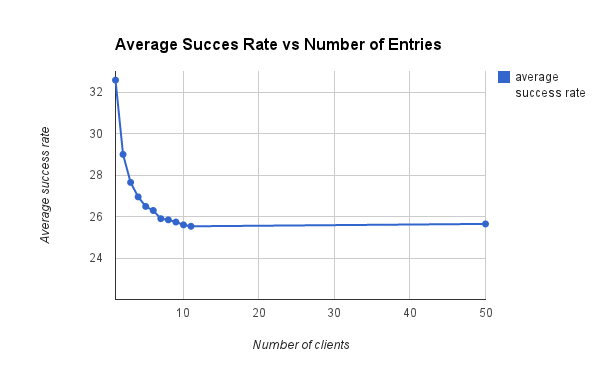
\includegraphics[scale=0.4]{exp3.jpg}
\caption{Result obtained with the 3rd eperiment, with drop = 10}
\end{center}
\end{figure}

\begin{figure}[h!]
\begin{center}
\hspace*{-1in}
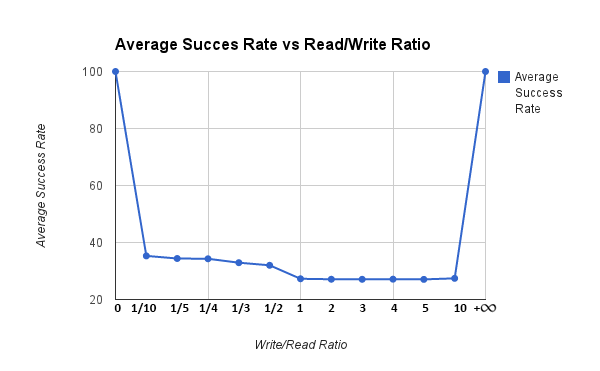
\includegraphics[scale=0.4]{exp4.jpg}
\caption{Result obtained with the 3rd eperiment, with drop = 3}
\end{center}
\end{figure}
 
\begin{figure}[h!]
\begin{center}
\hspace*{-1in}
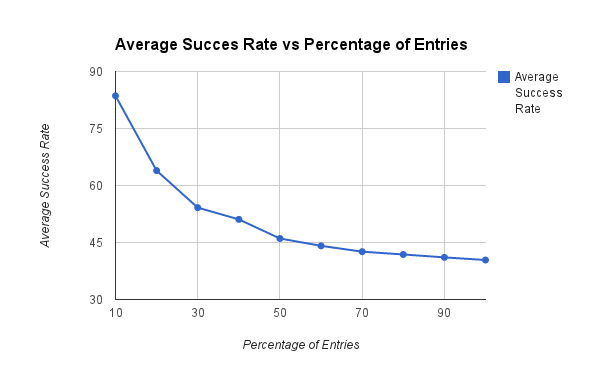
\includegraphics[scale=0.4]{exp5.jpg}
\caption{Result obtained with the 3rd eperiment, with drop = 2}
\end{center}
\end{figure}



\subsection{Increase the number of proposers and acceptors}
We now want to see what happens when we increase the number of proposers and acceptors. We first tried to increase only the number of proposers (from 3 to 6), then only the number of acceptors (from 5 to 9) and then both. We just need to add the following code to the file paxy.erl.
\begin{lstlisting}
-define(RED, {255,0,0}).
-define(BLUE, {0,0,255}).
-define(GREEN, {0,255,0}).
-define(YELLOW, {255,255,0}).
-define(CYAN, {0,255,255}).
-define(MAGENTA, {255,0,255}).

% Sleep is a list with the initial sleep time for each proposer
start(Sleep) ->
    AcceptorNames = ["Acceptor 1", "Acceptor 2", "Acceptor 3", "Acceptor 4", "Acceptor 5", "Acceptor 6", "Acceptor 7", "Acceptor 8", "Acceptor 9"],
    AccRegister = [a, b, c, d, e, f, g, h, i],
    ProposerNames = ["Proposer 1", "Proposer 2", "Proposer 3","Proposer 4", "Proposer 5", "Proposer 6"],
    PropInfo = [{kurtz, ?RED}, {kilgore, ?GREEN}, {willard, ?BLUE}, {hicks, ?YELLOW}, {johnson, ?CYAN}, {miller, ?MAGENTA}],
\end{lstlisting}
We made the experiment with drop = 3, so we have to compare with the 3 rounds we needed to find a consensus with 3 proposers and 5 acceptors. When we add more proposers, we see that we need 4 rounds, so a bit more. When we add more acceptors, we need 11 rounds. Finally, when we add both the algorithm terminates in 3 rounds so it seems that the number of round depends on the raio between proposers and acceptors.
\begin{figure}[h!]
\begin{center}
\hspace*{-1in}
\includegraphics[scale=0.4]{exp6.jpg}
\caption{Result obtained with 5 proposers}
\end{center}
\end{figure}

\begin{figure}[h!]
\begin{center}
\hspace*{-1in}
\includegraphics[scale=0.4]{exp7.jpg}
\caption{Result obtained with 9 acceptors}
\end{center}
\end{figure}
 
\begin{figure}[h!]
\begin{center}
\hspace*{-1in}
\includegraphics[scale=0.4]{exp8.jpg}
\caption{Result obtained with 5 proposers and 9 acceptors}
\end{center}
\end{figure}

\subsection{Split the Paxy module}

\section{Open questions}

\textit{Try to answer all the open questions in the documentation. When possible, do experiments to support your answers.}

\section{Personal opinion}

\textit{Provide your personal opinion of the seminar, including whether it should be included in next year's course or not.}

\end{document}
